% !TeX program = xelatex
\documentclass[10pt,aspectratio=169,xcolor=dvipsnames]{beamer}
\usepackage{fontspec}
\setmainfont{Arial}
\setsansfont{Arial}
\setmonofont{Arial}
\usepackage{amsmath,amssymb,amsthm,mathtools}
\usepackage{bm}
\usepackage{booktabs}
\usepackage{array}
\usepackage{colortbl}
\usepackage{tikz}
\usetikzlibrary{arrows.meta,positioning,shapes.geometric,fit,backgrounds,calc}
\usepackage{xcolor}
\usepackage{siunitx}

\hfuzz=60pt
\vfuzz=60pt
\hbadness=10000
\vbadness=10000

% ---- Theme ----
\usetheme{metropolis}
\usecolortheme{default}
\setbeamercolor{frametitle}{bg=NavyBlue!85!black,fg=white}
\setbeamercolor{progress bar}{fg=NavyBlue}
\setbeamerfont{frametitle}{size=\large,series=\bfseries}
\setbeamertemplate{navigation symbols}{}

% ---- Math macros ----
\newcommand{\PL}{\mathrm{PL}}
\newcommand{\HPL}{\mathrm{HPL}}
\newcommand{\VPL}{\mathrm{VPL}}
\newcommand{\HAL}{\mathrm{HAL}}
\newcommand{\VAL}{\mathrm{VAL}}
\newcommand{\IR}{\mathrm{IR}}
\newcommand{\FIM}{\mathrm{FIM}}
\newcommand{\E}{\mathbb{E}}
\newcommand{\1}{\mathbb{1}}
\newcommand{\R}{\mathbb{R}}
\newcommand{\diag}{\mathrm{diag}}
\newcommand{\tr}{\mathrm{tr}}
\newcommand{\Hset}{\mathcal{H}}
\newcommand{\Fset}{\mathcal{F}}
\newcommand{\hlb}[1]{\colorbox{yellow!35}{\(\displaystyle #1\)}}
\newcommand{\innov}[1]{\textcolor{NavyBlue}{\textbf{#1}}}

\title{\texorpdfstring{Integrity-Aware Autonomous Navigation for UAVs\\
\large Stage 1 Report: Architecture, Modules, and Contributions}{Integrity-Aware Autonomous Navigation for UAVs - Stage 1 Report}}
\subtitle{Integrity-Aware Autonomous Navigation with PL Field Predictor}
\author{\texorpdfstring{[Your Name]\\\small Supervisor: [Advisor Name]}{[Your Name] / Supervisor: [Advisor Name]}}
\institute{\small [Laboratory / Department]}
\date{\today}

\begin{document}

\maketitle

\begin{frame}{Outline}
  \tableofcontents
\end{frame}

% ========================================================
\section{Ch1 Background and Core Problem}
% ========================================================

\begin{frame}{1.1 Background: Integrity Requirements for Safety-Critical Autonomy}
  \begin{columns}[T]
    \column{.55\textwidth}
    \textbf{Status quo of the three-layer autonomy stack}
    \begin{itemize}\small
      \item \textbf{Estimation}: VIO / LIO / GNSS-INS fusion can already provide
        \(\hat{x}_k\) and covariance \(\Sigma_k\)
      \item \textbf{Planning}: EGO-Planner, Fast-Planner consume \textbf{mean estimates}
        \(\hat{x}_k\) and are largely unaware of covariance and faults
      \item \textbf{Control}: Geometric control / MPC are mature
    \end{itemize}
    \vspace{3pt}
    \textbf{New requirements in safety-critical scenarios}\\
    Urban low-altitude logistics, inspection, and emergency rescue
    $\Rightarrow$ require not only \textbf{high accuracy},
    but also \textbf{a known error bound} (bounded error guarantee)

    \column{.45\textwidth}
    \textbf{Aviation lesson: ARAIM}\\
    GNSS already has a mature \innov{Advanced RAIM} framework:
    \[
      P\bigl(|\epsilon| > \PL\bigr) \le \IR_{req} \approx 10^{-7}/h
    \]
    but it is not yet standardized for UAV multi-sensor fusion.

    \vspace{6pt}
    \begin{block}{\small Position of this work}
      \small Upgrade ARAIM \emph{protection level (PL)} from
      \textbf{a monitoring tool} to
      \textbf{a planning metric}.
    \end{block}
  \end{columns}
\end{frame}

\begin{frame}{1.2 Three Key Research Gaps}
  \begin{table}
    \small
    \begin{tabular}{p{0.18\textwidth} p{0.38\textwidth} p{0.38\textwidth}}
      \toprule
      \textbf{Gap} & \textbf{Current status} & \textbf{Strategy in this work}\\
      \midrule
      \textbf{Information flow} & SLAM covariance \(\Sigma_k\) is discarded by the planner;
      the planner uses only the mean state to construct ESDF collision costs &
      Introduce \(\PL\) as a \innov{first-class SLAM-to-planner metric}\\
      \addlinespace
      \textbf{Methodology} & ARAIM is mature for GNSS-only systems;
      GNSS+LiDAR+IMU has no agreed fault tree &
      Propose \innov{dual-source ARAIM}: GNSS fault atom + LiDAR factor-block fault atom, with shared statistical semantics\\
      \addlinespace
      \textbf{Spatiotemporal dimension} & ARAIM gives \textbf{pointwise PL at the current time and position};
      the planner needs a PL field at \textbf{future times and candidate positions} &
      Design \innov{PL Field Predictor}: a local 3D scalar field \(\PL(\bm{p})\), queried by A* and B-spline optimization\\
      \bottomrule
    \end{tabular}
  \end{table}

  \vspace{6pt}
  \footnotesize These three gaps point to the same issue: \textbf{there is no differentiable, queryable, and certifiable bridge between integrity metrics and motion planning}.
\end{frame}

\begin{frame}{1.3 Core Research Question and Scope of This Report}
  \begin{alertblock}{Core question (one sentence)}
    \textbf{How can the protection level produced by the localization module become a first-class planning signal, so that a UAV actively avoids low-integrity regions while preserving real-time performance and certifiability?}
  \end{alertblock}

  \vspace{8pt}
  \textbf{Stage 1 scope (this report)}
  \begin{itemize}\small
    \item \checkmark~Discrete-time FGO + decoupled planning architecture
    \item \checkmark~Dual-source ARAIM (GNSS + LiDAR VGICP factor block)
    \item \checkmark~PL Field Predictor + PI cost injection into EGO-Planner
    \item \checkmark~\innov{ROS2-based SO3 UAV simulation} with EGO-Planner, SO3 controller, GNSS simulator, LiDAR/IMU simulation, and IAP odometry feedback (PX4 SITL: future integration)
  \end{itemize}

  \textbf{Stage 2 scope (not covered in this report)}
  \begin{itemize}\small
    \item \(\times\)~Continuous-time B-spline joint MAP optimization
    \item \(\times\)~Explicit active perception (FIM \(\log\det\) cost directly in planning)
    \item \(\times\)~Modifying the SLAM factor graph to absorb planning costs
  \end{itemize}
\end{frame}

\begin{frame}{1.4 Contribution Positioning: U1--U4 Taxonomy}
  \footnotesize
  \begin{table}
    \begin{tabular}{p{0.18\textwidth} p{0.45\textwidth} c}
      \toprule
      \textbf{Level} & \textbf{Meaning} & \textbf{This work}\\
      \midrule
      U1 joint-opt & SLAM factor graph and planning cost jointly optimized & $\times$ (Stage 2)\\
      U2 tightly-coupled & Planning cost feeds back to modify SLAM structure & $\times$ (Stage 2)\\
      \rowcolor{yellow!25}
      U3 implicit active & Planning cost senses future information and guides the trajectory & \checkmark (weak form)\\
      \rowcolor{yellow!25}
      U4 metric-unified & SLAM and planner share the same metric (PL) & \checkmark (strong form)\\
      \bottomrule
    \end{tabular}
  \end{table}

  \vspace{6pt}
  \begin{block}{One-sentence positioning}
    \small This work implements \innov{strong-form U4 + weak-form U3}:
    Using PL as the shared metric, it implicitly guides the UAV through high-integrity regions while retaining the engineering and certification advantages of estimation--planning decoupling.
  \end{block}
\end{frame}

% ========================================================
\section{Ch2 Overall Architecture and Design Principles}
% ========================================================

\begin{frame}{2.1 Overall Data Flow (End-to-End Architecture)}
  \begin{center}
    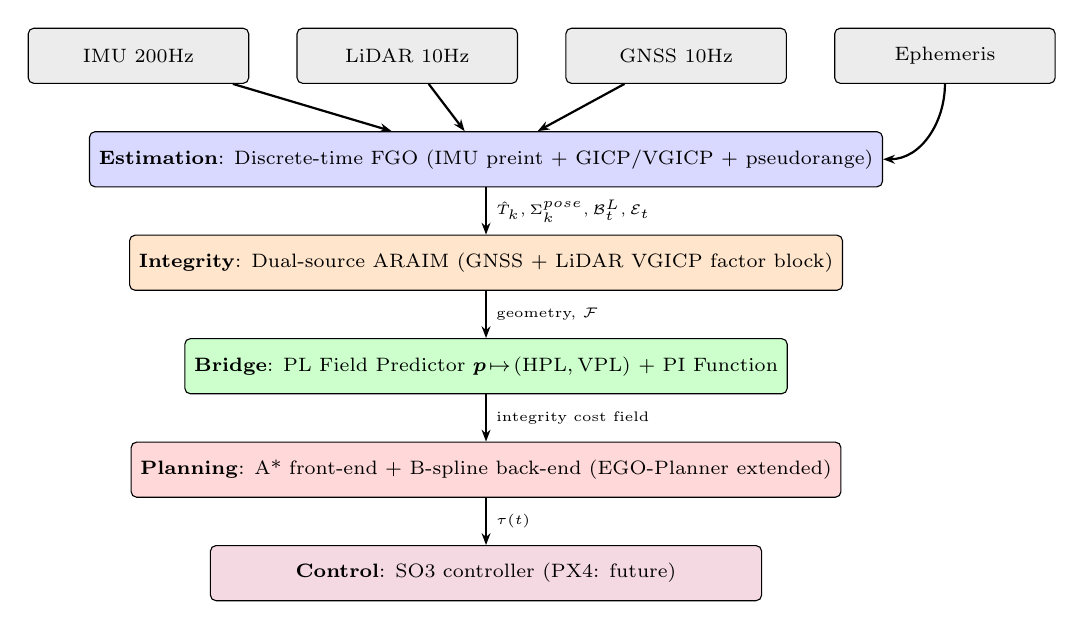
\begin{tikzpicture}[
        node distance=2.6mm and 6mm,
        box/.style={draw,rounded corners=2pt,minimum width=28mm,minimum height=7mm,font=\scriptsize,align=center},
        sens/.style={box,fill=gray!15},
        est/.style={box,fill=blue!15},
        intg/.style={box,fill=orange!20},
        br/.style={box,fill=green!20},
        plan/.style={box,fill=red!15},
        ctrl/.style={box,fill=purple!15},
        arr/.style={-{Stealth[length=1.5mm]},thick}
      ]
      \node[sens] (imu) {IMU 200Hz};
      \node[sens,right=of imu] (lidar) {LiDAR 10Hz};
      \node[sens,right=of lidar] (gnss) {GNSS 10Hz};
      \node[sens,right=of gnss] (eph) {Ephemeris};

      \node[est,below=6mm of lidar,xshift=10mm,minimum width=70mm] (fgo)
      {\textbf{Estimation}: Discrete-time FGO (IMU preint + GICP/VGICP + pseudorange)};

      \node[intg,below=6mm of fgo,minimum width=70mm] (araim)
      {\textbf{Integrity}: Dual-source ARAIM (GNSS + LiDAR VGICP factor block)};

      \node[br,below=6mm of araim,minimum width=70mm] (pred)
      {\textbf{Bridge}: PL Field Predictor $\bm{p}\!\mapsto\!(\HPL,\VPL)$ + PI Function};

      \node[plan,below=6mm of pred,minimum width=70mm] (planner)
      {\textbf{Planning}: A* front-end + B-spline back-end (EGO-Planner extended)};

      \node[ctrl,below=6mm of planner,minimum width=70mm] (ctl)
      {\textbf{Control}: SO3 controller (PX4: future)};

      \draw[arr] (imu) -- (fgo);
      \draw[arr] (lidar) -- (fgo);
      \draw[arr] (gnss) -- (fgo);
      \draw[arr] (eph.south) to[out=-90,in=0] (fgo.east);
      \draw[arr] (fgo) -- node[right,font=\tiny]{$\hat{T}_k,\Sigma^{pose}_k,\mathcal{B}^L_t,\mathcal{E}_t$} (araim);
      \draw[arr] (araim) -- node[right,font=\tiny]{geometry, $\Fset$} (pred);
      \draw[arr] (pred) -- node[right,font=\tiny]{integrity cost field} (planner);
      \draw[arr] (planner) -- node[right,font=\tiny]{$\tau(t)$} (ctl);
    \end{tikzpicture}
  \end{center}
  \centering\footnotesize
  Five-layer stack; modules are decoupled through explicit data contracts.
\end{frame}

\begin{frame}{2.2 Three Core Design Principles}
  \begin{block}{Principle 1: Estimation--Planning Decoupling + Metric Unification}
    \small SLAM and the planner are \textbf{not} jointly optimized, but they \textbf{share} the PL metric.
    Corresponds to strong-form U4. Clear certification/debugging advantages.
  \end{block}

  \begin{block}{Principle 2: Strict Separation Between Certified Monitoring and Advisory Prediction}
    \small
    \begin{itemize}\tiny
      \item ARAIM = \textbf{true} integrity decision at the current pose (designed to be certifiable under WG-C / DO-229 logic)
      \item PL Predictor = \emph{advisory} integrity prediction at candidate positions (for planning)
      \item Shared statistical models, but decoupled in function and code path
    \end{itemize}
  \end{block}

  \begin{block}{Principle 3: Local Rolling PL Cache (Off by Default, Demo-Enabled)}
    \small \innov{Code default}: \texttt{use\_grid=false}, resolution \(1\,\si{\meter}\),
    box \(30\times 30\times 8\,\si{\meter}\), max-age \(2.0\,\si{\second}\).
    In demo11, the grid is enabled via \texttt{phase2\_use\_pl\_grid=true}.
    The planner queries \(\widehat{\PL}(\bm{p})\) by trilinear interpolation and falls back to 0 (advisory cost off) if the field is stale, missing, or out of range.
  \end{block}
\end{frame}

\begin{frame}{2.3 Inter-Module Data Contracts (Interface Contracts)}
  \scriptsize
  \begin{table}
    \begin{tabular}{lllcc}
      \toprule
      \textbf{From} & \textbf{To} & \textbf{Payload (actual)} & \textbf{Rate} & \textbf{Path}\\
      \midrule
      Sensors & SLAM & raw IMU/LiDAR/GNSS & 10--200\,Hz & certified\\
      SLAM & ARAIM & $\hat{T}_t$, $\Sigma^{pose}_{t,6\times 6}$, $\mathcal{B}^L_t$, GNSS epoch & 10\,Hz & certified\\
      SLAM+ARAIM & PL Predictor & visible sats, $\Sigma^{pose}_{t,6\times 6}$, $\mathcal{B}^L_t$ summary & 2--10\,Hz & advisory\\
      PL Predictor & PI Module & local field $(\HPL,\VPL)(\bm{p})$ & 2\,Hz & advisory\\
      PI Module & Planner & \texttt{/iap/integrity\_front\_cost\_field} & 2\,Hz & advisory\\
      PI Module & Planner & \texttt{/iap/integrity\_cost\_field} (back-end) & 2\,Hz & advisory\\
      ARAIM & Supervisor & alarm flag $\1[\PL_k > \mathrm{AL}]$ & 10\,Hz & \innov{certified}\\
      Planner & Controller & B-spline $\tau(t)$ & 10--50\,Hz & --\\
      \bottomrule
    \end{tabular}
  \end{table}

  \vspace{6pt}
  \textbf{Three engineering values of the contract design:}
  \begin{itemize}\small
    \item \textbf{Replaceable}: any module can be replaced by a black box (e.g., FGO replaced by MSCKF) as long as it satisfies the contract
    \item \textbf{Parallelizable}: the Predictor runs in an independent thread and does not block the planner
    \item \textbf{Certifiable}: certified and advisory paths are physically separated
  \end{itemize}
\end{frame}

% ========================================================
\section{Ch3 Localization Module: GNSS+LiDAR+IMU Tightly Coupled FGO}
% ========================================================

\begin{frame}{3.1 Factor-Graph Structure (Baseline Infrastructure)}
  \scriptsize
  \textbf{State (full estimator state)}:
  \[
    \bm{x}_k =
    [\,\bm{T}_k,\ \bm{v}_k,\ \bm{b}^a_k,\ \bm{b}^g_k,\
    \delta t_k^{clk},\ \dot{\delta t}_k^{clk}\,]
  \]
  where \(\delta t^{clk}\) and \(\dot{\delta t}^{clk}\) are the GNSS receiver clock bias and drift, jointly estimated with pose, velocity, and IMU biases.

  \medskip
  MAP objective:
  \[
    \hat{\bm{X}} = \arg\min_{\bm{X}} \sum_{k}\Bigl\{
      \|r^{\mathrm{IMU}}_{k,k+1}\|^2_{\Sigma_I} +
      \sum_{F_{j,\ell}\in\Fset_L}\|r^{\mathrm{VGICP}}_{k,j,\ell}\|^2_{R_{j,\ell}} +
      \sum_{s \in \mathcal{S}_k}\|r^{\mathrm{GNSS}}_{k,s}\|^2_{\sigma_{URA,s}^2}
      + \|r^{\mathrm{prior}}_0\|^2_{\Sigma_0}
    \Bigr\}
  \]

  \textbf{LiDAR residual (actual: GICP/VGICP factor block)}:
  \[
    \bm{r}^{gicp}_{m} = \bm{T}_k\,\bm{p}_m - \bm{q}_m, \qquad
    \Sigma_m^{gicp} = \Sigma_m^{map} + \bm{R}_k\,\Sigma_m^{scan}\,\bm{R}_k^\top
  \]
  The point-to-plane form is a simplified explanatory case; the current IAP implementation primarily exposes \emph{direct GICP/VGICP matching factor blocks} \(F_{j,\ell}\) (target frame \(j\), voxelmap level \(\ell\)) to the integrity layer.

  \textbf{GNSS pseudorange residual (corrected)}:
  \[
    r^{\mathrm{GNSS}}_{k,s} = \rho_{k,s} -
    \bigl(\|\bm{P}_{ecef} - \bm{p}^W_{s,k}\| + \mathrm{Sagnac}
    + c\cdot\delta t_k^{clk} + I_s + T_s + \mathrm{TGD}_s\cdot c\bigr)
  \]
  where $\bm{P}_{ecef} = \bm{R}_{ext}\,\bm{p}_k^{body} + \bm{T}_{ecef}$ converts
  the local position to ECEF, Sagnac is the Earth-rotation correction,
  $I_s$ and $T_s$ are ionospheric (Klobuchar) and tropospheric (Saastamoinen)
  delays, and $\mathrm{TGD}_s$ is the transmitter group delay.

  \medskip
  \begin{alertblock}{Positioning of this chapter}
    \footnotesize This module is \textbf{not the main novelty of this work}. We use a mature architecture (LIO-style + tightly coupled GNSS) as the data source for the downstream integrity layer. The novelty starts from Ch4.
  \end{alertblock}
\end{frame}

\begin{frame}{3.2 Downstream Data Contract (Snapshot \(\mathcal{S}_t\))}
  \small
  Every 100 ms, the estimator publishes one snapshot to the Integrity Layer:
  \[
    \mathcal{S}_t =
    \bigl\{\hat{\bm{T}}_t,\ \Sigma^{p}_{t},\ \Sigma^{pose}_{t,6\times 6},\
    \mathcal{E}_t,\ \mathcal{B}^L_t,\ \mathcal{T}_t\bigr\}
  \]

  \begin{table}
    \scriptsize
    \begin{tabular}{lp{0.6\textwidth}}
      \toprule
      \textbf{Symbol} & \textbf{Meaning}\\
      \midrule
      $\hat{\bm{T}}_t$ & current MAP pose estimate (also \texttt{frame.sigma\_p} fallback)\\
      $\Sigma^{p}_{t}$ & 3$\times$3 position covariance (always available)\\
      $\Sigma^{pose}_{t,6\times 6}$ & 6$\times$6 pose covariance, optional via \texttt{FGOPositionInfo} or \texttt{LidarAraimSnapshot}\\
      $\mathcal{E}_t$ & visible-satellite epoch \{$s, \bm{p}^W_s, \sigma_{URA,s}, el_s, az_s$\}\\
      $\mathcal{B}^L_t$ & VGICP block snapshot list \{$F_{j,\ell}$, RMSE, inlier frac, $\kappa$, age\}\\
      $\mathcal{T}_t$ & trunk / TDOP detection summary used by the monitor\\
      \bottomrule
    \end{tabular}
  \end{table}

  \vspace{6pt}
  \textbf{Note on the information matrix}: the integrity layer does \textbf{not} consume a full $15\!\times\!15$ Hessian. The LiDAR ARAIM internally reconstructs $\Lambda_0$ from the 6$\times$6 pose covariance block, which is already sufficient for the snapshot-downdate hypothesis test (Ch 4.5).
  The estimator may maintain additional GNSS clock states internally; only the pose / position covariance block is exposed to the advisory path.
\end{frame}

% ========================================================
\section{Ch4 Dual-Source ARAIM \\(Core Contribution 1)}
% ========================================================

\begin{frame}{4.1 Standard ARAIM Recap (Blanch et al. MHSS)}
  \small
  \textbf{Fault-hypothesis set}:
  \[
    \Hset = \{H_0\} \cup \{H_s : s \in \mathcal{S}\} \cup \{H_c : c \in \mathcal{C}\}
  \]

  \textbf{Subset solution under each hypothesis}: $\hat{\bm{p}}_f = (G_f^\top W_f G_f)^{-1} G_f^\top W_f \bm{y}_f$, with covariance $\sigma_{q,f}^2 = [(G_f^\top W_f G_f)^{-1}]_{qq}$.

  \textbf{Solution Separation Test}: $|\hat{p}_{q,0} - \hat{p}_{q,f}| \le T_{q,f}$, otherwise raise an alarm.

  \medskip
  \textbf{Protection-level family used in this work} (consistent with Ch 4.5 and the actual code):
  \[
    \PL_{q,0} = K_{ff}\,\sigma_{q,0}
  \]
  \[
    \hlb{
      \PL_{q,f} = |d_{q,f}| + K_{fa,f}\,\sigma_{ss,q,f} + K_{md,f}\,\sigma_{q,f} + b_{q,f},
      \qquad
      \PL_q = \max\!\bigl(\PL_{q,0},\ \max_{f\ne 0}\PL_{q,f}\bigr)
    }
  \]
  where $d_{q,f}$ is the observed solution separation, $\sigma_{ss,q,f}$ is the separation standard deviation, $\sigma_{q,f}$ is the subset variance, and $b_{q,f}$ is the bias overbound for hypothesis $f$.

  \medskip
  \textbf{Integrity-risk equation (risk-budget allocation)}:
  \[
    \IR = P(H_0)\,P_{md|H_0} + \sum_{f\ne 0} P_{fault,f}\,P_{md|H_f} \le \IR_{req}
  \]

  \footnotesize
  where \(K_{fa}\) comes from false-alarm allocation and \(K_{md}\) from missed-detection allocation $P_{md|H_f}\le \IR_{req}/(M\cdot P_{fault,f})$.
\end{frame}

\begin{frame}{4.2 GNSS ARAIM Implementation in This System}
  \small
  \textbf{Configurable fault library}. The current implementation uses configurable per-satellite and per-constellation fault priors. The WG-C-style values below are used as \emph{reference defaults}; they must be verified/calibrated before any certification-level claim.

  \begin{table}\scriptsize
    \begin{tabular}{lll}
      \toprule
      Fault type & Default $P_{fault}$ & Note\\
      \midrule
      Single-satellite (GPS/Galileo) & $10^{-5}$ & Reference default\\
      Single-satellite (GLONASS/BDS) & $10^{-4}$ & More conservative reference\\
      Constellation (per system) & $10^{-4}$ & Reference default\\
      \bottomrule
    \end{tabular}
  \end{table}

  \textbf{Canopy-aware noise model (elevation-dependent)}:
  \[
    \sigma_{eff,s}^2(el_s,\kappa_s) = \sigma_0^2 + \frac{\sigma_{mp}^2}{\sin^2(el_s)} + \sigma_c^2 \cdot \exp\!\Bigl(\frac{\alpha\cdot\kappa_s}{\sin(el_s)}\Bigr)
  \]
  where $\kappa_s\in[0,1]$ is the ray-cast canopy density along the satellite line-of-sight.
  When $\kappa_s=0$ (open sky), the model reduces to elevation-dependent noise
  $\sigma_{eff}^2 = \sigma_0^2 + \sigma_{mp}^2/\sin^2(el_s) + \sigma_c^2$.
  Defaults: $\sigma_0=1.0\,\si{\meter}$, $\sigma_{mp}=0.5\,\si{\meter}$,
  $\sigma_c=5.0\,\si{\meter}$, $\alpha=2.0$.

  \medskip
  \textbf{Bias overbound (target model)}: $b_s = B_{nom} + B_{max,obs}$,
  where $B_{nom}$ is taken from WG-C as a reference default, and $B_{max,obs}$ is the design target derived from innovation-tail statistics. \emph{Strict per-constellation calibration of these terms is treated as future work.}
\end{frame}

\begin{frame}{4.3 LiDAR ARAIM: From Black-Box ICP to Factor-Block Integrity}
  \scriptsize

  \begin{alertblock}{Key distinction from conventional LiDAR integrity monitoring}
    \scriptsize
    IAP does \textbf{not} treat LiDAR ICP as a black-box pose measurement.
    Instead, the multi-scan VGICP matching cost is inserted into the FGO backend
    as direct factor blocks. Therefore, the LiDAR fault atom should follow the
    \innov{internal factor-block structure} rather than individual points or a
    post-ICP pose factor.
  \end{alertblock}

  \vspace{3pt}
  \textbf{Conventional ICP-as-pose-factor abstraction}
  \[
    r_{\mathrm{ICP}}=\log\!\left(\hat{T}_{\mathrm{ICP}}^{-1} T_k\right),
    \qquad
    \Delta\Lambda_{\mathrm{ICP}}=J_{\mathrm{ICP}}^\top R_{\mathrm{ICP}}^{-1}J_{\mathrm{ICP}}
  \]
  This abstraction hides which scan, keyframe, or resolution level caused the risk.

  \vspace{4pt}
  \textbf{IAP direct multi-scan VGICP factor abstraction}
  \[
    F_{j,\ell}=\mathrm{VGICPMatchingFactor}\bigl(
    \mathrm{source}=\mathcal{S}_t,\;\mathrm{target}=j,\;\mathrm{level}=\ell\bigr),
    \qquad
    \mathcal{F}_L=\{F_{j,\ell}\mid j\in\mathcal{T}_t,\ \ell\in\mathcal{L}\}
  \]

  \begin{block}{\small Consequence}
    \scriptsize
    The natural LiDAR ARAIM unit is not a single point, not a single plane, and
    not an ICP pose factor. It is a \innov{VGICP factor block} indexed by
    \((\mathrm{source},\mathrm{target},\mathrm{level})\).
  \end{block}
\end{frame}

\begin{frame}{4.4 IAP LiDAR Fault-Hypothesis Library}
  \scriptsize

  \textbf{LiDAR fault library induced by the VGICP block structure}
  \[
    \mathcal{H}_L
    =
    \{H_0,\ H_{\mathrm{source}}\}
    \cup
    \{H_{\mathrm{target}}(j):j\in\mathcal{T}_t\}
    \cup
    \{H_{\mathrm{level}}(\ell):\ell\in\mathcal{L}\}.
  \]

  \vspace{2pt}
  \begin{table}
    \scriptsize
    \begin{tabular}{p{0.20\textwidth} p{0.38\textwidth} p{0.34\textwidth}}
      \toprule
      \textbf{Fault mode} & \textbf{Meaning} & \textbf{Removed VGICP blocks}\\
      \midrule
      \(H_{\mathrm{source}}\)
      & Current deskewed source scan is unreliable
      & \(\mathcal{B}(H_{\mathrm{source}})=\{F_{j,\ell},\forall j,\ell\}\)\\
      \addlinespace
      \(H_{\mathrm{target}}(j)\)
      & Target frame / keyframe \(j\) is inconsistent
      & \(\mathcal{B}(H_{\mathrm{target}}(j))=\{F_{j,\ell},\forall \ell\}\)\\
      \addlinespace
      \(H_{\mathrm{level}}(\ell)\)
      & Voxelmap resolution level \(\ell\) is unreliable
      & \(\mathcal{B}(H_{\mathrm{level}}(\ell))=\{F_{j,\ell},\forall j\}\)\\
      \bottomrule
    \end{tabular}
  \end{table}

  \vspace{3pt}
  \textbf{Interpretation}
  \begin{itemize}\scriptsize
    \item \(H_{\mathrm{source}}\): dynamic contamination, deskew failure, poor current scan quality.
    \item \(H_{\mathrm{target}}(j)\): wrong historical keyframe pose, corrupted target map, large viewpoint inconsistency.
    \item \(H_{\mathrm{level}}(\ell)\): coarse level gives biased geometry, fine level becomes noisy or unstable.
  \end{itemize}

  \begin{alertblock}{\small Innovation}
    \scriptsize
    The LiDAR fault tree is not manually invented. It is induced by the actual
    IAP VGICP factor organization: \(\mathrm{source}\times\mathrm{target}\times\mathrm{level}\).
  \end{alertblock}
\end{frame}

\begin{frame}[t]{4.5 Snapshot Downdate: Real-Time LiDAR Subset ARAIM}
  \tiny
  \vspace{-2pt}
  \setlength{\abovedisplayskip}{2pt}
  \setlength{\belowdisplayskip}{2pt}
  \setlength{\abovedisplayshortskip}{1pt}
  \setlength{\belowdisplayshortskip}{1pt}
  \setlength{\jot}{0pt}

  \textbf{Linearized contribution of one VGICP block}
  \[
    (J_{j,\ell}, r_{j,\ell}, R_{j,\ell})=\mathrm{linearize}\bigl(F_{j,\ell},\hat{x}_0\bigr)
  \]
  \[
    \Delta\Lambda_{j,\ell}=J_{j,\ell}^{\top}R_{j,\ell}^{-1}J_{j,\ell},
    \qquad
    \Delta g_{j,\ell}=J_{j,\ell}^{\top}R_{j,\ell}^{-1}r_{j,\ell}
  \]

  \vspace{1pt}
  \textbf{Subset system under LiDAR fault hypothesis \(H_f\)}
  \[
    \Lambda_f=\Lambda_0-\sum_{F_{j,\ell}\in\mathcal{B}(H_f)}\Delta\Lambda_{j,\ell},
    \qquad
    g_f=g_0-\sum_{F_{j,\ell}\in\mathcal{B}(H_f)}\Delta g_{j,\ell}
  \]
  \[
    \delta x_f=\Lambda_f^{-1}g_f,\quad
    \hat{x}_f=\hat{x}_0\boxplus\delta x_f,\quad
    \Sigma_f=\Lambda_f^{-1}
  \]

  \vspace{1pt}
  \textbf{Solution separation and LiDAR protection level}
  \[
    d_f=\hat{x}_0\boxminus\hat{x}_f,\qquad
    \sigma_{q,f}=\sqrt{e_q^\top \Sigma_f e_q}
  \]
  \[
    T_{q,f}=K_{fa,f}\,\sigma_{ss,q,f},
    \qquad
    \PL^{L}_{q,f}=|e_q^\top d_f|+T_{q,f}+K_{md,f}\,\sigma_{q,f}+b_{q,f}
  \]
  \[
    \hlb{
      \PL^{L}_{q}=\max_{f\in\mathcal{H}_L}\PL^{L}_{q,f}
    }
  \]

  \vspace{-2pt}
  \begin{block}{\scriptsize Real-time design decision}
    \fontsize{5.7pt}{6.2pt}\selectfont
    We do \textbf{not} rerun the nonlinear smoother for every LiDAR hypothesis.
    We use the current linearized FGO snapshot and perform information-matrix
    downdate, which is compatible with online ARAIM timing.
  \end{block}
\end{frame}

\begin{frame}[t]{4.6 ICP/VGICP Quality as Integrity Evidence (Current vs Future)}
  \scriptsize
  \vspace{-2pt}
  \setlength{\abovedisplayskip}{3pt}
  \setlength{\belowdisplayskip}{3pt}
  \setlength{\abovedisplayshortskip}{2pt}
  \setlength{\belowdisplayshortskip}{2pt}

  \textbf{Current implementation (\texttt{block\_risk\_score()})}: a four-term normalized weighted sum
  {\footnotesize
    \[
      \gamma_{j,\ell} = w_r\,\frac{\mathrm{RMSE}_{j,\ell}}{\mathrm{RMSE}_{ref}}
      + w_i\,(1 - \mathrm{InlierFrac}_{j,\ell})
      + w_c\,\log\kappa_{j,\ell}
      + w_a\,\frac{\mathrm{Age}_j}{\mathrm{Age}_{ref}}
  \]}
  \begin{itemize}\tiny
      \setlength{\itemsep}{0.5pt}
    \item \(\mathrm{RMSE}_{j,\ell}\): VGICP residual RMS (\texttt{rmse\_proxy})
    \item \(\mathrm{InlierFrac}_{j,\ell}\): inlier ratio of the block
    \item \(\kappa_{j,\ell}\): condition-number / degeneracy proxy (\texttt{cond\_proxy})
    \item \(\mathrm{Age}_j\): temporal/topological age of target keyframe (\texttt{age\_sec})
  \end{itemize}

  \textbf{Current fault-prior model (mode-level, configurable)}:
  {\footnotesize
    \[
      P_{\mathrm{fault}}(H_{\mathrm{source}}) = p_{\mathrm{source}},\quad
      P_{\mathrm{fault}}(H_{\mathrm{target}}(j)) = p_{\mathrm{target}},\quad
      P_{\mathrm{fault}}(H_{\mathrm{level}}(\ell)) = p_{\mathrm{level}}
  \]}
  \tiny \(\gamma_{j,\ell}\) updates a \texttt{gamma\_mode} indicator that scales the bias overbound, not \(P_{\mathrm{fault}}\).

  \textbf{Bias overbound (current)}:
  {\footnotesize
    \[
      b_{q,H_{\mathrm{target}}(j)}=\alpha_q\max_{\ell}\gamma_{j,\ell},\quad
      b_{q,H_{\mathrm{level}}(\ell)}=\alpha_q\max_{j}\gamma_{j,\ell},\quad
      b_{q,H_{\mathrm{source}}}=\alpha_q\max_{j,\ell}\gamma_{j,\ell}
  \]}

  \begin{alertblock}{\scriptsize Future extension / calibratable model}
    \tiny
    A learned per-block prior using deskew error, dynamic-point ratio, and normal-distribution symmetry:
    {\footnotesize
      \[
        P_{\mathrm{fault},j,\ell} = \mathrm{clip}\!\left(\sigma\!\bigl(a_0 + a_1\gamma + a_2\,\mathrm{Dyn} + a_3\,\mathrm{Sym}\bigr)\right)
    \]}
    \(\mathrm{DeskewErr}\), \(\mathrm{Dyn}\), \(\mathrm{Sym}\) and the sigmoid mapping are \emph{not} in the current \texttt{block\_risk\_score()} / \texttt{enumerate\_hypotheses()}; they are Stage-2 calibration extensions.
  \end{alertblock}
\end{frame}

\begin{frame}[t]{4.7 Dual-Source Fusion Strategy (Conservative Fusion)}
  \scriptsize
  \vspace{-2pt}
  \setlength{\abovedisplayskip}{3pt}
  \setlength{\belowdisplayskip}{3pt}
  \setlength{\abovedisplayshortskip}{2pt}
  \setlength{\belowdisplayshortskip}{2pt}
  After computing the two PL channels independently, the runtime monitor performs a per-axis conservative max over $\PL_{E/N/U}$, then updates $\HPL$/$\VPL$ from the dominating source:
  {\footnotesize
    \[
      \PL_q^{\mathrm{fused}}=\max\!\bigl(\PL_q^{\mathrm{GNSS}},\PL_q^{\mathrm{LiDAR}}\bigr).
  \]}

  \textbf{Why conservative max instead of a joint fault tree?}
  \begin{itemize}\tiny
      \setlength{\itemsep}{1pt}
    \item \textbf{Conservatism}: the fused PL never underestimates risk from either channel
    \item \textbf{Decoupling}: GNSS and LiDAR fault libraries can evolve independently
    \item \textbf{Real-time}: complexity is additive, not combinatorial
    \item \textbf{Certifiability path}: minimal modification to the certified channel
  \end{itemize}

  \vspace{1pt}
  \begin{alertblock}{\scriptsize Risk-budget interpretation (rationale, \emph{not} an implemented metric)}
    \tiny
    At a paper level, the fused-risk upper bound is
    {\footnotesize
      \[
        \IR^{\mathrm{fused}}\le \IR^{\mathrm{GNSS}}+\IR^{\mathrm{LiDAR}}-\IR^{\mathrm{GNSS}}\IR^{\mathrm{LiDAR}}
        \approx \IR^{\mathrm{GNSS}}+\IR^{\mathrm{LiDAR}}.
    \]}
    This is a theoretical upper-bound rationale for the conservative max. The runtime monitor fuses $\PL/\HPL/\VPL$ and the dominating source label, but does \textbf{not} emit an explicit fused-IR scalar.
  \end{alertblock}

  \tiny \textbf{Complexity}: a joint sensor-fault tree scales as $\mathcal{O}(2^{|\mathcal{S}|+|\mathcal{B}|})$; conservative max scales as $\mathcal{O}(|\mathcal{S}|+|\mathcal{B}|)$, suitable for online UAV planning.
\end{frame}

\begin{frame}{4.8 Positioning Relative to Mainstream Work}
  \scriptsize
  \begin{table}
    \begin{tabular}{p{0.25\textwidth} p{0.22\textwidth} p{0.12\textwidth} p{0.14\textwidth} p{0.15\textwidth}}
      \toprule
      \textbf{Method} & \textbf{Fault enumeration} & \textbf{Multi-sensor} & \textbf{Real-time} & \textbf{Feeds planner}\\
      \midrule
      Blanch 2015 (MHSS) & GNSS satellite / constellation & $\times$ & \checkmark & $\times$\\
      Joerger \& Pervan 2019 & Sensor + satellite & \checkmark & partial & $\times$\\
      LiDAR RAIM / map RAIM & Landmark / map feature & partial & \checkmark & $\times$\\
      \rowcolor{yellow!25}
      \textbf{This work} & \textbf{GNSS + IAP VGICP block} & \textbf{\checkmark} & \textbf{\checkmark} & \textbf{\checkmark}\\
      \bottomrule
    \end{tabular}
  \end{table}

  \vspace{6pt}
  \begin{block}{Ch4 Contributions}
    \small
    \begin{enumerate}
      \item \textbf{Factor-aware LiDAR ARAIM}: extend ARAIM from satellite faults to IAP VGICP factor-block faults.
      \item \textbf{Structured LiDAR fault atoms}: source scan, target keyframe, voxelmap resolution level.
      \item \textbf{Snapshot downdate}: avoid rerunning the nonlinear FGO for every LiDAR hypothesis.
      \item \textbf{ICP-quality-driven bias overbound}: residual tail, inlier ratio, degeneracy, and target age.
      \item \textbf{Conservative GNSS--LiDAR fusion}: real-time feasibility, no combinatorial joint fault tree.
    \end{enumerate}
  \end{block}
\end{frame}

% ========================================================
\section{Ch5 PL Field Predictor \\ (Core Contribution 2)}
% ========================================================

\begin{frame}{5.1 Motivation: Why Is ARAIM Not Enough?}
  \small
  \textbf{Three mismatches}:

  \begin{enumerate}
    \item \textbf{Temporal mismatch}: ARAIM gives \(\PL(\bm{p}_t,t)\), the planner needs \(\PL(\bm{p}_{t+\Delta},t+\Delta)\), $\Delta\in[0.5,5]\,\si{\second}$.
    \item \textbf{Spatial mismatch}: ARAIM is a scalar at the current point, while the planner needs a \textbf{field} \(\PL:\R^3\to\R_+\).
    \item \textbf{Computational infeasibility}: embedding full MHSS into every B-spline gradient evaluation $\Rightarrow$ one replan $\approx n_{cp}\!\cdot n_{iter}\!\cdot T_{MHSS}\!=\!20\!\cdot\!50\!\cdot\!5\,\si{\milli\second}\!=\!5\,\si{\second}$, infeasible.
  \end{enumerate}

  \medskip
  \textbf{Design conclusion}: ARAIM online computation and planner-side queries must be \textbf{decoupled}.
  $\Rightarrow$ a \textbf{precomputed local scalar field} + \textbf{fast interpolation query interface}.

  \begin{block}{\small Role of the PL Field Predictor}
    \small A \innov{lightweight surrogate} of ARAIM in \textbf{space and future time}, used \textbf{only} on the advisory path.
  \end{block}
\end{frame}

\begin{frame}{5.2 Formal Module Definition}
  \small
  \textbf{Domain (default code parameters)}: a local box centered at the current UAV position $\bm{p}_t^0$:
  \[
    \Omega_t = \bm{p}_t^0 + [-L_x/2,L_x/2]\times[-L_y/2,L_y/2]\times[-L_z/2,L_z/2]
  \]
  \innov{Code defaults}: \(L_x=L_y=30\,\si{\meter}\), \(L_z=8\,\si{\meter}\), resolution \(1\,\si{\meter}\), max-age \(2.0\,\si{\second}\), \texttt{use\_grid=false}. Demo11 launch overrides these via \texttt{phase2\_use\_pl\_grid=true} and \texttt{phase2\_pl\_model=gnss\_geometry\_araim}.

  \medskip
  \textbf{Range and mapping}:
  \[
    \mathcal{P}_t:\Omega_t\to\R_{\ge 0}^2,\qquad
    \bm{p}\mapsto\bigl(\HPL(\bm{p}),\ \VPL(\bm{p})\bigr)
  \]

  \medskip
  \textbf{Decomposition into five serial submodules}:
  \[
    \bm{p}\xrightarrow{A}v_s(\bm{p})\xrightarrow{B}\Delta\Lambda_L(\bm{p})\xrightarrow{C}\Lambda_{pred}(\bm{p})\xrightarrow{D}\PL(\bm{p})\xrightarrow{E}\text{cached grid}
  \]

  \textbf{Key properties (Section 5.4)}:
  \begin{itemize}\scriptsize
    \item \textbf{Local Lipschitz continuity}: $|\PL(\bm{p}_1)-\PL(\bm{p}_2)|\le L_{\PL}\|\bm{p}_1-\bm{p}_2\|$
    \item \textbf{Self-consistency}: $\widehat{\PL}(\bm{p}_t^0)\approx \PL_{\mathrm{ARAIM}}(\bm{p}_t^0)$
  \end{itemize}
\end{frame}

\begin{frame}{5.3 Submodule A: Satellite Geometry Predictor}
  \small
  \textbf{Function}: given a candidate position $\bm{p}$, estimate the visible-satellite set and geometry at future time $t+\Delta$.

  \medskip
  \textbf{Visibility indicator}:
  \[
    v_s(\bm{p},t+\Delta)=\1\!\bigl[el_s(\bm{p},t+\Delta)>el_{min}\bigr]\cdot\1\!\bigl[\text{LoS}(\bm{p},\bm{p}^W_s(t+\Delta))\text{ unblocked}\bigr]
  \]

  \textbf{Elevation computation} (satellite positions extrapolated from $\mathcal{E}_t$):
  \[
    el_s(\bm{p},t+\Delta)=\arcsin\!\left(\frac{(\bm{p}^W_s(t+\Delta)-\bm{p})^\top\bm{u}_{up}(\bm{p})}{\|\bm{p}^W_s(t+\Delta)-\bm{p}\|}\right)
  \]

  \textbf{LoS blockage test} (optional): raycast in the occupancy map; in map-free scenes set $\text{LoS}=1$.

  \medskip
  \textbf{Geometry matrix}:
  \[
    G(\bm{p})=
    \begin{bmatrix}-\bm{e}_{s_1}^\top(\bm{p}) & 1\\\vdots & \vdots\\-\bm{e}_{s_N}^\top(\bm{p}) & 1
    \end{bmatrix},
    \quad
    \bm{e}_s(\bm{p})=\frac{\bm{p}^W_s-\bm{p}}{\|\bm{p}^W_s-\bm{p}\|}
  \]
  Retain only rows with $v_s(\bm{p})=1$.
\end{frame}

\begin{frame}{5.3 Submodule B: LiDAR Information Predictor (Optional)}
  \small
  \textbf{Function}: estimate the LiDAR information gain at candidate position $\bm{p}$.

  \textbf{Code default}: \texttt{use\_lidar\_observability=false}, i.e.\ this submodule is \emph{off by default}. When enabled, it acts as a confidence modulator on the current LiDAR information block.

  \medskip
  \textbf{Lightweight surrogate ($\alpha_L$ modulator)}:
  \[
    \hlb{
      \Delta\Lambda_{\mathrm{LiDAR}}(\bm{p})=\alpha_L(\bm{p})\cdot\Delta\Lambda_{\mathrm{LiDAR}}^{(t_0)}
    }
  \]
  where
  \begin{itemize}\scriptsize
    \item $\Delta\Lambda_{\mathrm{LiDAR}}^{(t_0)}$ is the actual LiDAR information contribution at the current time
    \item $\alpha_L(\bm{p})\in[0,1]$ is a \textbf{confidence modulator}, not a fault probability
  \end{itemize}

  \textbf{Modulator design} (point-density / condition-number based):
  \[
    \alpha_L(\bm{p})=\min\!\Bigl(1,\frac{N_{pts}(\bm{p})}{N_{good}}\Bigr)\cdot
    \min\!\Bigl(1,\frac{\kappa_{cond}^{ref}}{\kappa_{cond}(\bm{p})}\Bigr)
  \]
  \begin{itemize}\tiny
    \item $N_{pts}(\bm{p})$: LiDAR map points within search radius at $\bm{p}$; $N_{good}=80$
    \item $\kappa_{cond}(\bm{p})$: condition number of local geometry; $\kappa_{cond}^{ref}=30$
    \item $N_{pts}<N_{min}=12$ or $\kappa_{cond}>\kappa_{cond}^{max}$: fallback to $\alpha_L=0$
  \end{itemize}

  \footnotesize
  \textbf{Engineering rationale}: future positions have no source scan; the confidence modulator captures local geometric quality (density + conditioning) at near-zero cost. When the local point cloud is sparse or degenerate, $\alpha_L\to0$ and the fused-FIM PL falls back to GNSS-only.
\end{frame}

\begin{frame}{5.3 Submodule C: Fused FIM Assembler (Design Decision 2)}
  \small
  \textbf{Basic assembly}:
  \[
    \Lambda_{pred}^{(0)}(\bm{p})=\Lambda_{base}+\Delta\Lambda_{\mathrm{GNSS}}(\bm{p})+\alpha_L(\bm{p})\,\Delta\Lambda_{\mathrm{LiDAR}}^{(t_0)}
  \]

  \textbf{GNSS information contribution (position-dependent)}:
  \[
    \Delta\Lambda_{\mathrm{GNSS}}(\bm{p})=G^\top(\bm{p})\,W(\bm{p})\,G(\bm{p}),\quad
    W(\bm{p})=\diag\!\bigl(1/\sigma_{URA,s}^2(el_s(\bm{p}))\bigr)
  \]

  \medskip
  \begin{alertblock}{\small \innov{Position-dependent lightweight covariance growth (current code)}}
    \small
    The current \texttt{PredictedIntegrityComputer::sigma\_grow\_at()} only depends on visible-satellite deficit and mean canopy density:
    \[
      \hlb{
        \sigma_{grow}(\bm{p})=\sigma_0\!\left[1+\beta_v\,\frac{N_{nom}-N_{vis}(\bm{p})}{N_{nom}}+\beta_\kappa\,\bar{\kappa}(\bm{p})\right]
      }
    \]
    \scriptsize
    \begin{itemize}
      \item Term 1: visible-satellite-deficit penalty
      \item Term 2: mean canopy / GDOP-degeneracy proxy ($\bar\kappa$)
      \item \textcolor{gray}{Optional extension (not enabled in current code)}: a distance-anchor term $\beta_d\|\bm{p}-\bm{p}_t^0\|$ to penalize farther-from-anchor queries; reserved as a Stage 2 calibration knob.
    \end{itemize}
  \end{alertblock}

  \textbf{Final propagated covariance}:
  \[
    \Sigma_{pred}(\bm{p})=\bigl[\Lambda_{pred}^{(0)}(\bm{p})\bigr]^{-1}+\sigma_{grow}^2(\bm{p})\,\mathbf{I}_3
  \]
  This is the \textbf{engineering compromise} between frozen $\Sigma$ (too aggressive) and full FIM forward propagation (too expensive).
\end{frame}

\begin{frame}{5.3 Submodule D: GNSS Geometry-Only ARAIM PL + Optional Fused-FIM PL}
  \small
  \textbf{Current implementation (\texttt{PredictedAraimComputer::predict\_geometry()})}: \emph{geometry-only} mode.
  The Predictor predicts visible satellites from a candidate position, builds the geometry matrix $G(\bm{p})$, and calls a zero-residual ARAIM evaluator (no full per-grid MHSS over LiDAR hypotheses).

  \medskip
  \textbf{Compute fault-free protection level} (subset variance from $\Sigma_{pred}(\bm{p})$):
  \[
    \sigma_{q,0}^2(\bm{p})=\bigl[\Sigma_{pred}(\bm{p})\bigr]_{qq},\qquad
    \PL_{q,0}(\bm{p})=K_{ff}\,\sigma_{q,0}(\bm{p})+b_{q,0}(\bm{p})
  \]

  \textbf{For GNSS satellite hypotheses $f\in\Hset_{\mathrm{GNSS}}$} (with downdate $\Lambda_{pred}-\Delta\Lambda_f$):
  \[
    \PL_{q,f}(\bm{p})=K_{fa,f}\,\sigma_{ss,q,f}(\bm{p})+K_{md,f}\,\sigma_{q,f}(\bm{p})+b_{q,f}(\bm{p})
  \]

  \textbf{HPL / VPL}:
  \[
    \hlb{
      \HPL(\bm{p})=\max\!\Bigl(\PL_{h,0}(\bm{p}),\ \max_{f\in\Hset_{\mathrm{GNSS}}}\PL_{h,f}(\bm{p})\Bigr)
    }
  \]
  analogous form for $\VPL$.

  \medskip
  \textbf{Optional conservative fused-FIM PL} (when \texttt{use\_fused\_fim\_grid=true}): combine GNSS base information with the LiDAR-observability FIM, compute $\HPL^{\mathrm{fused}}$, and take per-axis max with the GNSS-only $\HPL$.

  \footnotesize
  \emph{Note}: the current Predictor exposes $\HPL(\bm{p})$ and $\VPL(\bm{p})$. A full $\IR(\bm{p})$ field over all LiDAR-source hypotheses is reserved as future work.
\end{frame}

\begin{frame}[t]{5.3 Submodule E: Field Cache \& Interpolator}
  \scriptsize
  \vspace{-2pt}
  \setlength{\abovedisplayskip}{3pt}
  \setlength{\belowdisplayskip}{3pt}
  \textbf{Grid storage (code defaults)}:
  \begin{itemize}\tiny
      \setlength{\itemsep}{1pt}
    \item Resolution $\Delta=1\,\si{\meter}$
    \item Size $30\times 30\times 8 = 7200$ voxels
    \item Each voxel stores $(\HPL,\VPL)\in\R^2$ plus risk-band metadata
    \item Total memory $\approx 60\,\si{\kilo\byte}$
  \end{itemize}

  \vspace{1pt}
  \textbf{Query interface} (trilinear interpolation):
  \[
    \widehat{\PL}(\bm{p})=\sum_{i=0}^{7}w_i(\bm{p})\,\PL(\bm{v}_i),\quad\sum_i w_i=1
  \]

  \textbf{Gradient (when needed by the back-end optimizer)}:
  \[
    \nabla_{\bm{p}}\widehat{\PL}(\bm{p})=\sum_{i=0}^{7}\bigl[\nabla_{\bm{p}}w_i(\bm{p})\bigr]\,\PL(\bm{v}_i)
  \]

  \vspace{1pt}
  \textbf{Update strategy}:
  \begin{itemize}\tiny
      \setlength{\itemsep}{1pt}
    \item Eager precompute around the UAV at 2\,Hz
    \item Lazy on-demand for first-touched voxels
    \item \innov{Field aging}: voxels older than \texttt{grid\_max\_age\_s}=2.0\,\si{\second} are \emph{stale}; the planner falls back to 0 advisory cost
  \end{itemize}
\end{frame}

\begin{frame}{5.4 Summary of Key Design Decisions (Engineering Contributions)}
  \footnotesize
  \begin{table}
    \begin{tabular}{p{0.20\textwidth} p{0.35\textwidth} p{0.35\textwidth}}
      \toprule
      \textbf{Decision} & \textbf{Full-FIM route} & \textbf{Route in this work}\\
      \midrule
      LiDAR future contribution & Virtual VGICP block ARAIM at every voxel & \innov{Optional $\alpha_L(\bm{p})$ confidence modulator (off by default)}\\
      Covariance forward propagation & Full Hessian propagation along trajectory & \innov{Position-dependent $\sigma_{grow}$ (visible-deficit + canopy)}\\
      ARAIM--Predictor coupling & Embedded shared computation graph & \innov{Functional decoupling, shared statistical model}\\
      Online subset enumeration & Full MHSS at every voxel & \innov{Geometry-only ARAIM at voxels; full MHSS only at the current pose}\\
      \bottomrule
    \end{tabular}
  \end{table}

  \medskip
  \begin{block}{\small Proposition 1 (self-consistency target)}
    \scriptsize At $\bm{p}=\bm{p}_t^0$, with proper calibration of $\beta_v,\beta_\kappa$, the Predictor satisfies
    \[
      \bigl|\widehat{\PL}(\bm{p}_t^0)-\PL_{\mathrm{ARAIM}}(\bm{p}_t^0)\bigr|\le \epsilon_0
    \]
    with $\epsilon_0\to 0$ when $\sigma_{grow}(\bm{p}_t^0)\to 0$. A formal closed-form conservatism bound is reserved as future work; numerical Monte-Carlo verification is used as the substitute (Ch 8.4).
  \end{block}
\end{frame}

\begin{frame}{5.5 Real-Time Design and Overall Timing}
  \small
  \begin{center}
    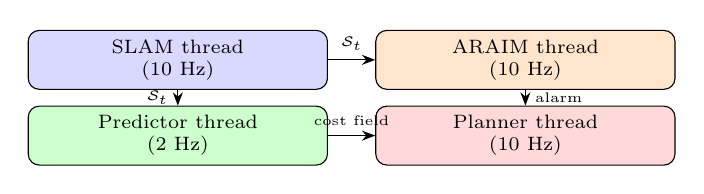
\begin{tikzpicture}[
        node distance=2mm and 6mm,
        thr/.style={draw,rounded corners,font=\scriptsize,minimum height=5mm,minimum width=38mm,align=center}
      ]
      \node[thr,fill=blue!15] (slam) {SLAM thread\\(10 Hz)};
      \node[thr,fill=orange!20,right=of slam] (araim) {ARAIM thread\\(10 Hz)};
      \node[thr,fill=green!20,below=of slam] (pred) {Predictor thread\\(2 Hz)};
      \node[thr,fill=red!15,right=of pred] (plan) {Planner thread\\(10 Hz)};

      \draw[-{Stealth}] (slam) -- node[above,font=\tiny]{$\mathcal{S}_t$} (araim);
      \draw[-{Stealth}] (slam) -- node[left,font=\tiny]{$\mathcal{S}_t$} (pred);
      \draw[-{Stealth}] (araim) -- node[right,font=\tiny]{alarm} (plan);
      \draw[-{Stealth}] (pred) -- node[above,font=\tiny]{cost field} (plan);
    \end{tikzpicture}
  \end{center}

  \medskip
  \textbf{Key timing constraints (with default $30\times 30\times 8$ box)}:
  \begin{itemize}\scriptsize
    \item One full Predictor scan over $7200$ voxels: $\le 200\,\si{\milli\second}$ on Intel i7-class CPU
    \item Planner replan period: $100\,\si{\milli\second}$; each replan queries $\sim 200$ points $\Rightarrow <5\,\si{\milli\second}$
    \item Field aging threshold: $2.0\,\si{\second}$ (\texttt{grid\_max\_age\_s})
  \end{itemize}

  \textbf{Degradation strategy (Graceful Degradation)}:
  \[
    c_{PI}(\bm{p})=
    \begin{cases}\pi(\HPL(\bm{p}),\VPL(\bm{p})), & \text{field fresh}\wedge \bm{p}\in\Omega_t\\ 0, & \text{field stale}\vee \bm{p}\notin\Omega_t
    \end{cases}
  \]

  \footnotesize $\Rightarrow$ If the Predictor fails or is disabled, the planner degrades to standard EGO-Planner without introducing additional risk.
\end{frame}

% ========================================================
\section{Ch6 PI Function and Two-Stage Cost Architecture (Core Contribution 3)}
% ========================================================

\begin{frame}{6.1 Role of the PI Function}
  \small
  \textbf{Definition}: a mapping from integrity metrics to planning cost
  \[
    \pi:\R_{\ge 0}^2\to\R_{\ge 0},\quad(\HPL,\VPL)\mapsto c_{PI}
  \]

  \medskip
  \textbf{Three invocation points in the system}:
  \begin{enumerate}\small
    \item \innov{Front-end A* edge cost} via \texttt{/iap/integrity\_front\_cost\_field}
    \item \innov{Back-end planner cost} via \texttt{/iap/integrity\_cost\_field}
    \item Safety Supervisor: $\1[\PL_k^{\mathrm{ARAIM}}>\mathrm{AL}]$ triggers a safety action
  \end{enumerate}

  \medskip
  \begin{alertblock}{\small Key Design Philosophy}
    \small The PI function uses \textbf{different forms} in the front-end and back-end:\\
    --- Front end: \(\pi_{front}\) is based on a \textbf{dimensionless ratio} and used as a \emph{multiplicative edge inflation}\\
    --- Back end: \(\pi_{back}\) is based on a \textbf{dimensional hinge} on AL margin\\
    Together, they form a \innov{two-stage cost architecture}---an architectural contribution of this work.
  \end{alertblock}
\end{frame}

\begin{frame}{6.2 Back End: B-spline Hinge-based PI Cost}
  \small
  B-spline trajectory: $\tau(t)=\sum_i B_i(t)\,\bm{c}_i$, control-point set $\{\bm{c}_i\}$.

  \medskip
  \textbf{PI cost (hinge squared)}:
  \[
    \hlb{
      J_{PI}^{back}(\tau)=\sum_i\Bigl\{w_H[\max(0,\HPL(\bm{c}_i)+m_H-\HAL)]^2+w_V[\max(0,\VPL(\bm{c}_i)+m_V-\VAL)]^2\Bigr\}
    }
  \]

  \medskip
  \begin{alertblock}{\small Implementation status (\emph{partial})}
    \scriptsize
    The hinge cost form is implemented in \texttt{PICostAdapter}. In the current pipeline, the planner consumes \emph{precomputed cost (and gradient when available) samples} from \texttt{/iap/integrity\_cost\_field}, rather than back-propagating $\nabla\HPL(\bm{c}_i)$ analytically inside the optimizer. Fully analytic PL-gradient back-propagation through the predictor is kept as a method-level extension.
  \end{alertblock}

  \medskip
  \textbf{Two improvements over standard $\pi_1$}:
  \begin{enumerate}\scriptsize
    \item \innov{Dynamic AL}: use mission-level $\HAL,\VAL$ (isomorphic to ARAIM)
    \item \innov{Explicit margin} $m_H,m_V$: build a buffer before the AL boundary
  \end{enumerate}

  \textbf{Typical values}: $\HAL=10\,\si{\meter}$, $\VAL=6\,\si{\meter}$, $m_H=1.5\,\si{\meter}$, $m_V=1.0\,\si{\meter}$, $w_H=w_V=2.0$.
\end{frame}

\begin{frame}[t]{6.3 Front End: A* Ratio-based PI Cost as Multiplicative Edge Inflation}
  \scriptsize
  \vspace{-2pt}
  \setlength{\abovedisplayskip}{3pt}
  \setlength{\belowdisplayskip}{3pt}
  \textbf{Define a dimensionless integrity occupancy ratio}:
  \[
    \hlb{
      r(\bm{p})=\max\!\left(\frac{\HPL(\bm{p})}{\HAL},\ \frac{\VPL(\bm{p})}{\VAL}\right)\in[0,\infty)
    }
  \]

  \textbf{Piecewise quadratic cost (risk band)}:
  \[
    c_{PI}^{front}(\bm{p})=
    \begin{cases}
      0, & r\le 0.7\quad\text{(SAFE)}\\
      \left(\dfrac{r-0.7}{0.3}\right)^2, & 0.7<r\le 1\quad\text{(CAUTION)}\\
      1+(r-1)^2, & r>1\quad\text{(ALARM)}
    \end{cases}
  \]

  \vspace{1pt}
  \textbf{\innov{A* edge cost (multiplicative inflation, current implementation)}}:
  \[
    \hlb{
      e(\bm{p}_i,\bm{p}_j)=\|\bm{p}_i-\bm{p}_j\|\cdot\bigl(1+\lambda_{front}\,c_{PI}^{front}(\bm{p}_j)\bigr)
    }
  \]
  where $c_{PI}^{front}(\bm{p}_j)$ is queried by nearest-neighbor lookup on the IntegrityCostMap; if the field is stale, missing, or out of radius, $c_{PI}^{front}=0$ and the edge degenerates to standard EGO geometry.

  \vspace{1pt}
  \textbf{Why a ratio (and why multiplicative)?}
  \begin{itemize}\tiny
    \item \textbf{Dimensionless}: ratio is independent of HAL/VAL absolute calibration
    \item \textbf{Heuristic-friendly}: multiplicative inflation preserves admissibility of the Euclidean heuristic
    \item \textbf{Zero interference in SAFE regions}: when $r\le 0.7$, behavior reduces to original EGO
    \item \textbf{Strong topology discrimination}: penalizes already in CAUTION, encouraging high-integrity corridors
  \end{itemize}
\end{frame}

\begin{frame}[t]{6.4 Engineering Value of the Two-Stage Architecture}
  \scriptsize
  \vspace{-2pt}
  \begin{table}
    \scriptsize
    \setlength{\tabcolsep}{3pt}
    \renewcommand{\arraystretch}{0.95}
    \begin{tabular}{p{0.13\textwidth} p{0.21\textwidth} p{0.18\textwidth} p{0.34\textwidth}}
      \toprule
      \textbf{Stage} & \textbf{Cost form} & \textbf{Complexity} & \textbf{Role}\\
      \midrule
      Front-end A* & Ratio, multiplicative edge inflation & $\mathcal{O}(1)$ per edge & \innov{Global topology guidance: avoid high-PL corridors}\\
      Back-end B-spline & Hinge squared, dimensional & $\mathcal{O}(n_{cp}\cdot n_{iter})$ & \innov{Local refinement: build margin at the AL boundary}\\
      \bottomrule
    \end{tabular}
  \end{table}

  \vspace{1pt}
  \textbf{Corresponding classic motion-planning paradigm}:
  \[
    \text{front-end heuristic search}+\text{back-end local optimization}
  \]
  \scriptsize Compatible with mainstream architectures such as Fast-Planner and EGO-Planner.

  \vspace{1pt}
  \begin{block}{\scriptsize Why not use a single cost everywhere?}
    \tiny
    \begin{itemize}
      \item Hinge only: front end may pick an average-high-PL corridor with every point still below HAL, which back end cannot recover
      \item Ratio only: dimensionless back-end cost conflicts with $J_{smooth}$ and $J_{collision}$ scales
    \end{itemize}
    $\Rightarrow$ \textbf{Separation of responsibilities} is architecturally necessary.
  \end{block}
\end{frame}

\begin{frame}{6.5 Graceful Degradation and Safety Supervisor}
  \small
  \textbf{Field health monitoring}:
  \[
    \mathrm{health}(t)=\1[t-t_{\text{last update}}<\texttt{grid\_max\_age\_s}]\cdot\frac{|\text{fresh voxels}|}{|\Omega_t|}
  \]

  \textbf{Automatic degradation strategy}:
  \[
    c_{PI}^{\text{effective}}(\bm{p})=\mathrm{health}(t)\cdot c_{PI}(\bm{p})
  \]

  \medskip
  \textbf{Safety Supervisor (engineering state machine, \texttt{IntegrityMonitor})}:
  \[
    \mathrm{State}(t)=
    \begin{cases}\texttt{UNSAFE}, & \PL_k\ge\mathrm{AL}\\\texttt{SAFE\_EXCLUDED}, & \text{fault detected}\wedge \PL_k<\mathrm{AL}\\\texttt{SAFE}, & \text{recovered after consecutive safe frames}
    \end{cases}
  \]

  When unsafe, the system executes one of:
  \begin{itemize}\scriptsize
    \item Decelerate/hover and recompute the front-end A* path
    \item Roll back to the trajectory from the most recent fresh field
    \item Trigger emergency landing
  \end{itemize}

  \begin{alertblock}{\small Certification perspective}
    \scriptsize The Supervisor remains \emph{independent} from the advisory Predictor and provides an \textbf{engineering safety fallback} based on the current ARAIM-style PL/AL monitor. \emph{Formal certification-level risk guarantees (full WG-C / DO-229 overbound proofs across all sensor error models) remain future work.}
  \end{alertblock}
\end{frame}

% ========================================================
\section{Ch7 Planning Module: EGO-Planner Extension}
% ========================================================

\begin{frame}{7.1 EGO-Planner Baseline Recap}
  \small
  \textbf{Original objective function} (Zhou et al. 2021):
  \[
    J_{EGO}=\lambda_s J_{smooth}+\lambda_c J_{collision}+\lambda_d J_{dynamic}
  \]

  \textbf{Smooth cost}: $J_{smooth}=\sum_i\|\bm{c}_i-2\bm{c}_{i+1}+\bm{c}_{i+2}\|^2$

  \textbf{Collision cost} (ESDF-based): $J_{collision}=\sum_i\bigl[\max(0,d_{thr}-d_{\mathrm{ESDF}}(\bm{c}_i))\bigr]^2$

  \medskip
  \textbf{Why choose EGO-Planner?}
  \begin{itemize}\scriptsize
    \item Decoupled architecture matches the discrete-time SLAM route in this work
    \item B-spline control points are the most natural injection point for PI cost
    \item ZJU-FAST-Lab open-source implementation is mature
    \item ESDF collision cost and PL hinge cost have isomorphic mathematical forms $\Rightarrow$ gradient templates can be reused
  \end{itemize}
\end{frame}

\begin{frame}{7.2 Optimization Problem After Integrity Extension}
  \small
  \textbf{Extended back-end objective}:
  \[
    \hlb{
      J_{total}=\lambda_s J_{smooth}+\lambda_c J_{collision}+\lambda_d J_{dynamic}+\lambda_\pi^{back} J_{PI}^{back}
    }
  \]

  \medskip
  \textbf{Front-end A* extension (multiplicative edge cost, matches IAP code)}:
  \[
    e(n,n')=\|\bm{p}_n-\bm{p}_{n'}\|\cdot\bigl(1+\lambda_{front}\,c_{PI}^{front}(\bm{p}_{n'})\bigr)+\lambda_o\,c_{\mathrm{occ}}(n')
  \]
  The Euclidean heuristic $h(n)$ is unchanged (admissibility preserved when $\lambda_{front}\ge 0$).

  \medskip
  \textbf{Typical hyperparameter values}:
  \begin{table}\scriptsize
    \begin{tabular}{llll}
      \toprule
      Parameter & Value & Parameter & Value\\
      \midrule
      $\lambda_s$ & 10.0 & $\lambda_{front}$ & 2.0\\
      $\lambda_c$ & 10000.0 & $\lambda_\pi^{back}$ & 2.0\\
      $\lambda_d$ & 0.01 & B-spline order & 3\\
      \bottomrule
    \end{tabular}
  \end{table}

  \textbf{Implementation note}: the back-end PI cost is formulated as a hinge loss; in the current implementation, the planner consumes \emph{precomputed cost/gradient samples} from the integrity cost field rather than back-propagating $\nabla\HPL$ analytically through the predictor. Fully analytic PL-gradient back-propagation is reserved as a method-level extension.
\end{frame}

\begin{frame}{7.3 Cross-Process IntegrityCostMap Communication Design}
  \small
  \textbf{Engineering choice}: do not fork the EGO-Planner source; communicate via ROS2 topics.

  \medskip
  \begin{center}
    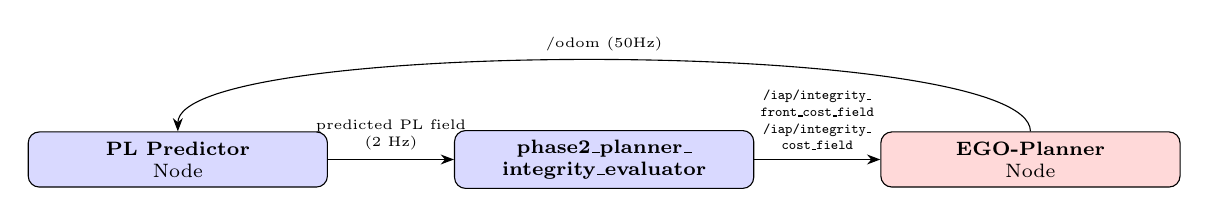
\begin{tikzpicture}[
        node distance=5mm and 16mm,
        proc/.style={draw,rounded corners,font=\scriptsize,minimum height=7mm,minimum width=38mm,align=center}
      ]
      \node[proc,fill=blue!15] (p1) {\textbf{PL Predictor}\\Node};
      \node[proc,fill=blue!15,right=of p1] (p2) {\textbf{phase2\_planner\_}\\\textbf{integrity\_evaluator}};
      \node[proc,fill=red!15,right=of p2] (p3) {\textbf{EGO-Planner}\\Node};

      \draw[-{Stealth}] (p1) -- node[above,font=\tiny,align=center]{predicted PL field\\(2 Hz)} (p2);
      \draw[-{Stealth}] (p2) -- node[above,font=\tiny,align=center]{\texttt{/iap/integrity\_}\\\texttt{front\_cost\_field}\\\texttt{/iap/integrity\_}\\\texttt{cost\_field}} (p3);
      \draw[-{Stealth}] (p3.north) .. controls +(0,12mm) and +(0,12mm) .. node[above,font=\tiny,align=center]{/odom (50Hz)} (p1.north);
    \end{tikzpicture}
  \end{center}

  \medskip
  \textbf{Two cost fields with distinct schemas}:
  \begin{itemize}\scriptsize
    \item \textbf{Front-end A* field} \texttt{/iap/integrity\_front\_cost\_field} (PointCloud2):
      \[
        \{x,y,z,\HPL,\VPL,\HAL,\VAL,\text{cost},\text{risk\_band\_code}\}
      \]
      consumed by EGO-Planner front-end A* via the multiplicative edge inflation in \S 7.2.
    \item \textbf{Back-end / evaluator field} \texttt{/iap/integrity\_cost\_field} (PointCloud2):
      $\{x,y,z,\text{cost},\text{grad}_x,\text{grad}_y,\text{grad}_z,\text{risk\_band}\}$ when gradient samples are available.
  \end{itemize}

  \textbf{Advantages}: no modification of EGO-Planner memory model; native RViz visualization (publish = debug); multiple subscribers (Supervisor also listens).
\end{frame}

% ========================================================
\section{Ch8 Experimental Validation}
% ========================================================

\begin{frame}{8.1 Simulation Platform and demo11 Scenario}
  \small
  \textbf{Platform (current main loop)}: \innov{ROS2-based SO3 UAV simulation} on Ubuntu / ROS2 Jazzy (Intel i7-class CPU). Key chain: \texttt{traj\_server}~$\to$~\texttt{SO3 controller}~$\to$~\texttt{SO3 plant}~$\to$~\texttt{IAP odom feedback}, with EGO-Planner, GNSS simulator, LiDAR/IMU simulation.\\
  \emph{PX4 SITL / Gazebo: planned future integration, not the current validation platform.}

  \medskip
  \textbf{demo11 ``Stratified Canopy'' scenario design}:
  \begin{itemize}\scriptsize
    \item Corridor length $\approx 100\,\si{\meter}$; lower-canopy density $\rho_{low}=0.1$, upper-canopy density $\rho_{up}=0.6$
    \item Left--right asymmetry: dense canopy on one side (heavy GNSS blockage), sparse on the other
    \item Expected behavior: UAV chooses the sparse-canopy corridor (better PL) over the geometric shortest path
  \end{itemize}

  \textbf{Run mode}: \texttt{use\_so3\_dynamics:=true}; demo11 enables \texttt{phase2\_use\_pl\_grid=true}, \texttt{phase2\_pl\_model=gnss\_geometry\_araim}.

  \textbf{Comparison configurations} (via launch flags):
  \begin{itemize}\scriptsize
    \item \emph{Baseline}: \texttt{planner\_use\_integrity\_cost=false}, \texttt{planner\_use\_integrity\_front\_search=false}
    \item \emph{Front-only}: \texttt{planner\_use\_integrity\_front\_search=true}
    \item \emph{Full}: above two enabled jointly with global integrity search
  \end{itemize}
\end{frame}

\begin{frame}{8.2 Completed Validation (Preliminary)}
  \small
  \textbf{Single-module functional smoke tests (\checkmark, qualitative)}:
  \begin{itemize}\scriptsize
    \item FGO+ARAIM stack runs end-to-end in demo11 without crash
    \item ARAIM HPL/VPL time-series rises during simulated GNSS blockage (qualitative trend matches expectation)
    \item PL Field Predictor visualization in RViz shows clear left--right anisotropy in stratified canopy
    \item PI cost is injected into EGO-Planner via \texttt{/iap/integrity\_front\_cost\_field}; closed-loop pipeline runs
  \end{itemize}

  \medskip
  \textbf{End-to-end closed loop (\checkmark, small-scale)}:
  \begin{itemize}\scriptsize
    \item Several demo11 closed-loop runs completed without runtime errors
    \item Visual inspection: trajectories under \emph{Full} configuration tend to bias toward the sparser-canopy side, while \emph{Baseline} traces a geometrically shorter line
  \end{itemize}

  \medskip
  \begin{alertblock}{\small Status: preliminary smoke tests / qualitative observations}
    \scriptsize
    Quantitative numbers (e.g., APE, peak HPL, success counts) are \emph{not yet} statistically validated. Large-scale benchmarking, log archiving, and CSV-based statistics are scheduled in the next two weeks (\S8.3, \S8.4).
  \end{alertblock}
\end{frame}

\begin{frame}{8.3 Baseline Comparison Experiment Design (Planned)}
  \small
  \textbf{Comparison configurations matching the README launch flags}:
  \begin{table}\scriptsize
    \begin{tabular}{lllll}
      \toprule
      ID & Description & Front edge cost & Back-end cost & Status\\
      \midrule
      B1 & Baseline (standard EGO) & off & off & primary control\\
      B2 & Front-only & ratio (multiplicative) & off & primary contrast\\
      \rowcolor{yellow!25}
      B4 & Full system (this work) & ratio (multiplicative) & hinge & primary target\\
      B3 & Back-end-only & off & hinge & \textbf{optional ablation}\\
      \bottomrule
    \end{tabular}
  \end{table}
  \scriptsize B1 / B2 / B4 are the three primary configurations directly supported by the README launch flags. B3 (back-end-only) is enabled only if the integrity back-end cost field is configured independently of the front-end injection.

  \medskip
  \textbf{Evaluation metrics}:
  \begin{table}\scriptsize
    \begin{tabular}{p{0.28\textwidth} p{0.48\textwidth} p{0.14\textwidth}}
      \toprule
      Metric & Definition & Expected\\
      \midrule
      Success rate & \# successful arrivals / \# total runs & $\uparrow$ B4\\
      Avg HPL / Max HPL & $\bar{\HPL}$ and $\max\HPL$ along the trajectory & $\downarrow$ B4\\
      Trajectory length & $\int\|\dot\tau\|\,\si{dt}$ & close to B1\\
      Replan compute time & average ms per replan & B4 $\le$ B1 + 20\%\\
      Supervisor trigger rate & \# Alarm / mission time & $\downarrow$ B4\\
      \bottomrule
    \end{tabular}
  \end{table}

  \textbf{Statistical test}: Mann--Whitney U on each metric pair, $\alpha=0.05$.
\end{frame}

\begin{frame}{8.4 Self-Consistency Sanity Check (Critical)}
  \small
  \textbf{Purpose}: verify that the Predictor matches the certified ARAIM at $\bm{p}=\bm{p}_t^0$.

  \medskip
  \textbf{Metric}:
  \[
    \epsilon_{self}(t)=\bigl|\widehat{\HPL}(\bm{p}_t^0)-\HPL^{\mathrm{ARAIM}}_t\bigr|/\HPL^{\mathrm{ARAIM}}_t
  \]

  \textbf{Acceptance target}:
  \[
    \E[\epsilon_{self}]<5\%,\quad\mathrm{P95}[\epsilon_{self}]<15\%
  \]
  (initial loose targets; tightened after $\sigma_{grow}$ calibration in W3)

  \medskip
  \textbf{Visualizations}:
  \begin{itemize}\scriptsize
    \item Scatter plot $\widehat{\HPL}(\bm{p}_t^0)$ vs $\HPL^{\mathrm{ARAIM}}_t$ (target: lie on $y=x$)
    \item Time-series overlay of the two curves
    \item Residual histogram (target: zero-mean, small variance)
  \end{itemize}

  \begin{alertblock}{\small Failure diagnosis}
    \scriptsize If $\epsilon_{self}$ stays above target: $\sigma_{grow}(0)$ is mis-calibrated (should approach 0 at $\bm{p}=\bm{p}_t^0$), or the constant component of $\alpha_L$ has not been zeroed.
  \end{alertblock}
\end{frame}

\begin{frame}{8.5 Scenario-Response Test Matrix (Planned)}
  \footnotesize
  \begin{table}
    \begin{tabular}{p{0.2\textwidth} p{0.32\textwidth} p{0.38\textwidth}}
      \toprule
      \textbf{Scenario} & \textbf{Key feature} & \textbf{Expected PL-field response}\\
      \midrule
      Open field & many satellites visible; sparse LiDAR features & nearly constant, near-isotropic; low HPL\\
      Urban canyon & vertical satellite blockage; lateral visibility & VPL rises in canyon; horizontal anisotropy\\
      Corridor (demo11) & LiDAR longitudinal weakness; GNSS variable & longitudinal HPL rise; lateral stable; strong anisotropy\\
      Tunnel entrance & GNSS visibility drops sharply & steep spatial gradient; CAUTION$\to$ALARM transition\\
      Stratified canopy & sparse/dense asymmetry & lower PL on sparse side $\Rightarrow$ B4 chooses sparse side\\
      \bottomrule
    \end{tabular}
  \end{table}

  \medskip
  \textbf{Validation method}:
  \begin{enumerate}\scriptsize
    \item Collect 2D slices of $\PL(\bm{p})$ in each scenario (qualitative match with physical intuition)
    \item Quantitative anisotropy ratio $\lambda_{max}/\lambda_{min}$ of the spatial gradient tensor
    \item Trajectory-shape comparison between B1 and B4
  \end{enumerate}
\end{frame}

% ========================================================
\section{Ch9 Summary and Next Steps}
% ========================================================

\begin{frame}{9.1 Core Contribution Checklist}
  \small
  \textbf{Positioning relative to U1--U4}:
  \begin{itemize}
    \item \innov{U4 (metric-unified)}: \checkmark \textbf{architecture completed}---PL is the shared SLAM-to-planner metric
    \item \innov{U3 (implicit active perception)}: \checkmark architecture completed, empirical validation ongoing
    \item U1 (joint optimization): $\times$ Stage 2
    \item U2 (tightly-coupled): $\times$ Stage 2
  \end{itemize}

  \medskip
  \textbf{Three claimable contributions (with honest scope statements)}:
  \begin{enumerate}\small
    \item \innov{Factor-aware LiDAR ARAIM}: VGICP factor-block fault library, snapshot downdate, ICP-quality-driven bias overbound; conservative max fusion with GNSS ARAIM
    \item \innov{Lightweight PL Field Predictor}: GNSS geometry-only ARAIM at voxels with optional fused-FIM PL, position-dependent $\sigma_{grow}$ surrogate, decoupled 2 Hz advisory thread
    \item \innov{Two-stage PI cost architecture}: front-end ratio-based \emph{multiplicative edge inflation} (topology) + back-end hinge cost (margin)
  \end{enumerate}

  \textbf{Underlying engineering contributions}:
  \begin{itemize}\scriptsize
    \item Physical separation between certified monitor and advisory predictor
    \item Cross-process IntegrityCostMap (\texttt{/iap/integrity\_*\_cost\_field}) without forking EGO-Planner
  \end{itemize}
\end{frame}

\begin{frame}{9.2 Completed Work Checklist (Honest Status)}
  \footnotesize
  \begin{table}
    \begin{tabular}{p{0.20\textwidth} p{0.55\textwidth} c}
      \toprule
      \textbf{Chapter} & \textbf{Work item} & \textbf{Status}\\
      \midrule
      Ch3 SLAM & FGO (IMU+VGICP+GNSS pseudorange) running in demo11 & \checkmark\\
      Ch3 SLAM & Snapshot $\mathcal{S}_t$ publishing interface (pose cov + block list) & \checkmark\\
      Ch4 ARAIM & GNSS MHSS implementation + URA model & \checkmark\\
      Ch4 ARAIM & LiDAR source/target/level fault hypotheses & \checkmark\\
      Ch4 ARAIM & LiDAR block risk score and bias overbound & \checkmark\\
      Ch4 ARAIM & Conservative GNSS--LiDAR max fusion & \checkmark\\
      Ch4 ARAIM & Learned per-block $P_{fault,b}$ (sigmoid + Dyn/Sym/DeskewErr) & \emph{future work}\\
      Ch5 Predictor & GNSS geometry-only ARAIM grid + optional fused-FIM PL & \checkmark\\
      Ch5 Predictor & Trilinear interpolation + field aging + degradation & \checkmark\\
      Ch5 Predictor & $\sigma_{grow}$ (visible-deficit + canopy) surrogate & \checkmark\\
      Ch5 Predictor & Full subset-MHSS / IR field over all source hypotheses & \emph{future work}\\
      Ch6 PI & Front-end ratio cost field (multiplicative edge inflation) & \checkmark\\
      Ch6 PI & Back-end hinge cost formulation / cost-field gradient interface & \emph{partial}\\
      Ch7 Planner & Decoupled EGO-Planner extension via ROS2 topics & \checkmark\\
      Ch8 Exp & demo11 closed-loop smoke tests (qualitative) & \checkmark\\
      Ch8 Exp & Large-scale 3-baseline comparison (B1/B2/B4, $\ge$ 60 runs) & \emph{ongoing}\\
      Ch8 Exp & Quantitative self-consistency sanity check & \emph{ongoing}\\
      Ch5 Theory & Closed-form conservatism proof of $\sigma_{grow}$ & \emph{future work; MC numerical substitute}\\
      \bottomrule
    \end{tabular}
  \end{table}
\end{frame}

\begin{frame}{9.3 Near-Term To-Do List (6-Week Rolling Plan)}
  \small
  \begin{table}
    \scriptsize
    \begin{tabular}{p{0.08\textwidth} p{0.42\textwidth} p{0.42\textwidth}}
      \toprule
      \textbf{Week} & \textbf{Task} & \textbf{Deliverable}\\
      \midrule
      W1 & demo11 B1/B2/B4 large-scale runs ($\ge$ 60 each), with logs & success-rate / PL / trajectory-length CSVs and figures\\
      W2 & Self-consistency sanity check + scenario-response slices & all figures for \S8.4 and \S8.5\\
      W3 & $\sigma_{grow}$ calibration report + $\alpha_L$ activation experiment & calibration document + before/after curves\\
      W4 & Paper draft (Method + Experiment) & draft v0.5\\
      W5 & UrbanNav qualitative replay (optional) + revision & draft v0.9\\
      W6 & Advisor review + submission (T-IV / ICRA / IROS) & submission\\
      \bottomrule
    \end{tabular}
  \end{table}

  \medskip
  \textbf{Key risks and mitigation}:
  \begin{itemize}\scriptsize
    \item Risk A: closed-form $\sigma_{grow}$ conservatism proof is intractable $\Rightarrow$ Monte-Carlo numerical validation
    \item Risk B: Predictor latency exceeds 200 ms with default box $\Rightarrow$ shrink box / lower resolution / reduce hypothesis enumeration
    \item Risk C: UrbanNav has no ground-truth PL $\Rightarrow$ qualitative-only, excluded from quantitative comparisons
    \item Risk D: PX4 SITL integration not on the critical path $\Rightarrow$ explicitly framed as future work
  \end{itemize}
\end{frame}

\begin{frame}{9.4 Stage 2 Outlook}
  \small
  \textbf{Three open problems from Stage 1 to Stage 2}:
  \begin{enumerate}
    \item \textbf{Joint MAP optimization} on continuous-time B-splines (U1)
      \[
        \min_{\{\bm{c}_i\}}\Bigl\{\underbrace{J_{MAP}^{SLAM}(\{\bm{c}_i\})}_{\text{factor graph}}+\lambda\,\underbrace{J_{plan}(\{\bm{c}_i\})}_{\text{smooth+collision+PI}}\Bigr\}
      \]
    \item \textbf{Explicit active perception} (strong-form U3)
      \[
        J_{active}=-\sum_i\log\det\!\bigl(\Lambda_{pred}(\bm{c}_i)\bigr)
      \]
    \item Let the SLAM factor graph absorb planning costs (U2)
  \end{enumerate}

  \medskip
  \textbf{Migration path}:
  \begin{itemize}\scriptsize
    \item PL Predictor reused, but upgraded from advisory to part of certified path
    \item $\sigma_{grow}$ surrogate replaced by full FIM forward propagation
    \item Predictor frequency drops from 10 Hz to 2 Hz, trading rate for U1 capability
    \item Learned per-block $P_{fault,b}$, deskew/dynamic/symmetry features brought online
  \end{itemize}
\end{frame}

\begin{frame}{9.5 Explicit Requests for Advisor Feedback}
  \small
  \textbf{Five questions for today's meeting}:

  \begin{enumerate}
    \item \textbf{Submission target}: For Stage 1, T-IV / ICRA / IROS---which fits best? Should we split into two papers (factor-aware LiDAR ARAIM + PL-Predictor planning architecture)?
    \item \textbf{Contribution ordering}: Among the three contributions, which should be the headline?
    \item \textbf{Experimental depth}: Are large-scale demo11 simulations sufficient, or is a real dataset (UrbanNav / M2DGR) required?
    \item \textbf{Boundary of theoretical proof}: If a closed-form conservatism proof for $\sigma_{grow}$ is intractable, is Monte-Carlo numerical validation acceptable?
    \item \textbf{Stage 2 prioritization}: Should all three Stage 2 directions (U1 / U2 / strong-form U3) be pursued, or focus on one as the PhD core contribution?
  \end{enumerate}

  \vspace{6pt}
  \begin{block}{}
    \centering\small Thank you for your attention --- Q \& A
  \end{block}
\end{frame}

\end{document}
